\section{Maxwell's Equations \& Wave Propagation}
\label{sec:maxwell}

\begin{nontechnical}
\textbf{Maxwell's Equations explain how every wireless device works}---from your phone to GPS satellites to radio telescopes.

\textbf{Simple idea:} Electric and magnetic fields can create each other. When they do this in just the right way, they form a wave that travels through space at the speed of light.

\textbf{The four rules:}
\begin{enumerate}
\item Electric charges create electric fields
\item Magnetic field lines always form closed loops (no magnetic monopoles)
\item Changing magnetic fields create electric fields (how generators work)
\item Electric currents and changing electric fields create magnetic fields (how antennas work)
\end{enumerate}

\textbf{Maxwell's breakthrough:} He realized these four rules predict waves traveling at exactly the speed of light---proving that light itself is an electromagnetic wave!

\textbf{Real impact:} Every wireless technology (WiFi, Bluetooth, 5G, GPS, radar, satellite TV) relies on electromagnetic waves described by these equations.
\end{nontechnical}

\section{Overview}

\textbf{Maxwell's Equations} are the fundamental laws of electromagnetism, unifying electricity, magnetism, and optics into a single coherent framework. Formulated by James Clerk Maxwell in 1865, these four elegant equations describe how electric and magnetic fields interact and propagate through space.

\begin{keyconcept}
Maxwell's Equations predict that electromagnetic disturbances propagate as \textbf{waves} at the speed of light, proving that light itself is an electromagnetic phenomenon. This unification of optics with electromagnetic theory represents one of the greatest achievements in physics.
\end{keyconcept}

\section{The Four Maxwell's Equations}

\subsection{Differential Form (Local Description)}

\subsubsection{1. Gauss's Law (Electric)}

\textbf{Electric charges create electric fields:}
\begin{equation}
\nabla \cdot \mathbf{E} = \frac{\rho}{\epsilon_0}
\label{eq:gauss-electric}
\end{equation}
where:
\begin{itemize}
\item $\mathbf{E}$ = electric field vector (V/m)
\item $\rho$ = charge density (C/m³)
\item $\epsilon_0 = 8.854 \times 10^{-12}$ F/m = permittivity of free space
\end{itemize}

\textbf{Physical meaning:} Electric field lines originate from positive charges and terminate on negative charges. The divergence of $\mathbf{E}$ at any point is proportional to the charge density there.

\subsubsection{2. Gauss's Law for Magnetism}

\textbf{No magnetic monopoles exist:}
\begin{equation}
\nabla \cdot \mathbf{B} = 0
\label{eq:gauss-magnetic}
\end{equation}
where:
\begin{itemize}
\item $\mathbf{B}$ = magnetic field vector (Tesla or Wb/m²)
\end{itemize}

\textbf{Physical meaning:} Magnetic field lines always form closed loops---there are no isolated north or south poles. Breaking a magnet in half creates two smaller magnets, each with both poles.

\subsubsection{3. Faraday's Law of Induction}

\textbf{Changing magnetic fields create electric fields:}
\begin{equation}
\nabla \times \mathbf{E} = -\frac{\partial \mathbf{B}}{\partial t}
\label{eq:faraday}
\end{equation}
where:
\begin{itemize}
\item $\nabla \times$ = curl operator (measures circulation/rotation)
\item $\partial \mathbf{B}/\partial t$ = time rate of change of magnetic field
\end{itemize}

\textbf{Physical meaning:} A time-varying magnetic field induces a circulating electric field. This is the fundamental principle behind electrical generators, transformers, and induction heating.

\begin{calloutbox}{Example: Electric Generator}
Spin a magnet near a coil of wire. The changing magnetic flux through the coil induces a circulating electric field (Eq.~\ref{eq:faraday}), which drives current through the wire. This converts mechanical energy to electrical energy.
\end{calloutbox}

\subsubsection{4. Ampère-Maxwell Law}

\textbf{Electric currents and changing electric fields create magnetic fields:}
\begin{equation}
\nabla \times \mathbf{B} = \mu_0 \mathbf{J} + \mu_0 \epsilon_0 \frac{\partial \mathbf{E}}{\partial t}
\label{eq:ampere-maxwell}
\end{equation}
where:
\begin{itemize}
\item $\mu_0 = 4\pi \times 10^{-7}$ H/m = permeability of free space
\item $\mathbf{J}$ = current density (A/m²)
\item $\mu_0 \epsilon_0 \partial \mathbf{E}/\partial t$ = \textbf{displacement current} (Maxwell's addition!)
\end{itemize}

\textbf{Physical meaning:} Moving charges (conduction current) AND time-varying electric fields both create circulating magnetic fields.

\begin{keyconcept}
\textbf{Maxwell's Critical Insight:} The displacement current term $\partial \mathbf{E}/\partial t$ was missing from Ampère's original law. Maxwell added it for mathematical consistency---and this single term predicts electromagnetic waves can exist! Without it, light would be impossible.
\end{keyconcept}

\section{Derivation of the Wave Equation}

\subsection{From Maxwell's Equations to Waves}

In free space (vacuum), with no charges ($\rho = 0$) and no currents ($\mathbf{J} = \mathbf{0}$), Maxwell's equations become:

\textbf{Step 1:} Take the curl of Faraday's Law (Eq.~\ref{eq:faraday}):
\begin{equation}
\nabla \times (\nabla \times \mathbf{E}) = -\nabla \times \left(\frac{\partial \mathbf{B}}{\partial t}\right) = -\frac{\partial}{\partial t}(\nabla \times \mathbf{B})
\label{eq:curl-faraday}
\end{equation}

\textbf{Step 2:} Substitute Ampère-Maxwell Law (Eq.~\ref{eq:ampere-maxwell}) with $\mathbf{J} = \mathbf{0}$:
\begin{equation}
\nabla \times (\nabla \times \mathbf{E}) = -\mu_0 \epsilon_0 \frac{\partial^2 \mathbf{E}}{\partial t^2}
\label{eq:curl-sub}
\end{equation}

\textbf{Step 3:} Use vector identity $\nabla \times (\nabla \times \mathbf{E}) = \nabla(\nabla \cdot \mathbf{E}) - \nabla^2 \mathbf{E}$

In vacuum with $\rho = 0$, Gauss's Law (Eq.~\ref{eq:gauss-electric}) gives $\nabla \cdot \mathbf{E} = 0$, so:
\begin{equation}
\boxed{\nabla^2 \mathbf{E} = \mu_0 \epsilon_0 \frac{\partial^2 \mathbf{E}}{\partial t^2}}
\label{eq:wave-E}
\end{equation}

\textbf{This is the wave equation for the electric field!}

\textbf{Step 4:} An identical derivation starting from the curl of Eq.~\ref{eq:ampere-maxwell} yields:
\begin{equation}
\boxed{\nabla^2 \mathbf{B} = \mu_0 \epsilon_0 \frac{\partial^2 \mathbf{B}}{\partial t^2}}
\label{eq:wave-B}
\end{equation}

\subsection{Wave Speed and the Speed of Light}

The general wave equation for a field $f$ is:
\begin{equation}
\nabla^2 f = \frac{1}{v^2} \frac{\partial^2 f}{\partial t^2}
\label{eq:wave-general}
\end{equation}
where $v$ is the wave propagation speed.

Comparing Eq.~\ref{eq:wave-E} with Eq.~\ref{eq:wave-general}:
\begin{equation}
\frac{1}{v^2} = \mu_0 \epsilon_0
\end{equation}

Therefore:
\begin{equation}
v = \frac{1}{\sqrt{\mu_0 \epsilon_0}} = \frac{1}{\sqrt{(4\pi \times 10^{-7})(8.854 \times 10^{-12})}} = 2.998 \times 10^8 \text{ m/s} = c
\label{eq:speed-of-light}
\end{equation}

\begin{keyconcept}
\textbf{Maxwell's Triumph:} The electromagnetic wave speed calculated from fundamental constants equals the measured speed of light! This proved that \textbf{light is an electromagnetic wave}---one of the greatest unifications in physics.
\end{keyconcept}

\section{Plane Wave Solutions}

\subsection{General Form}

For a plane wave propagating in the $+z$ direction, the electric and magnetic fields are:

\begin{equation}
\mathbf{E}(z,t) = E_0 \cos(kz - \omega t + \phi) \, \hat{\mathbf{x}}
\label{eq:plane-wave-E}
\end{equation}

\begin{equation}
\mathbf{B}(z,t) = B_0 \cos(kz - \omega t + \phi) \, \hat{\mathbf{y}}
\label{eq:plane-wave-B}
\end{equation}

where:
\begin{itemize}
\item $k = 2\pi/\lambda$ = wave number (rad/m)
\item $\omega = 2\pi f$ = angular frequency (rad/s)
\item $\lambda$ = wavelength (m)
\item $f$ = frequency (Hz)
\item $\phi$ = phase constant (rad)
\item $E_0, B_0$ = field amplitudes
\end{itemize}

\subsection{Relationship Between E and B}

The electric and magnetic field amplitudes are related by:
\begin{equation}
B_0 = \frac{E_0}{c}
\label{eq:E-B-relation}
\end{equation}

In general vector form:
\begin{equation}
\mathbf{B} = \frac{1}{c} \hat{\mathbf{k}} \times \mathbf{E}
\label{eq:E-B-vector}
\end{equation}
where $\hat{\mathbf{k}}$ is the unit vector in the propagation direction.

\begin{keyconcept}
\textbf{Transverse Wave Property:} $\mathbf{E}$ and $\mathbf{B}$ are perpendicular to each other AND to the propagation direction $\hat{\mathbf{k}}$. They oscillate in phase, with their magnitudes related by Eq.~\ref{eq:E-B-relation}.
\end{keyconcept}

\subsection{Electromagnetic Wave Visualization}

\begin{center}
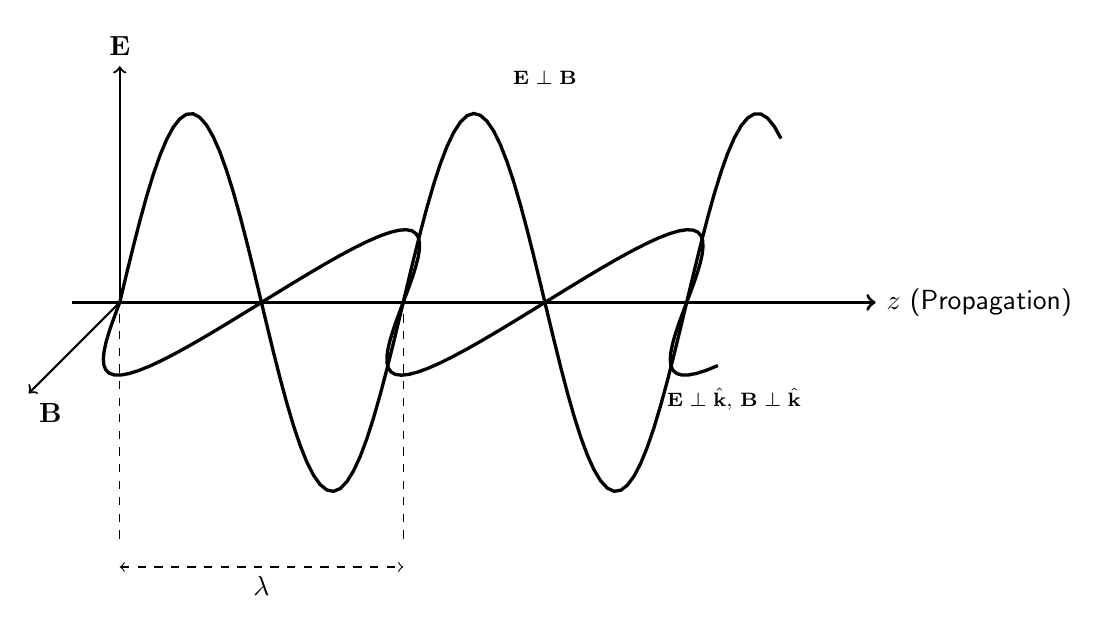
\begin{tikzpicture}[scale=1.2]
% Propagation direction axis
\draw[->,very thick] (-0.5,0,0) -- (8,0,0) node[right] {\sffamily $z$ (Propagation)};

% Electric field (vertical, red oscillation)
\draw[->,thick,black] (0,0,0) -- (0,2.5,0) node[above] {\sffamily $\mathbf{E}$};
\draw[very thick,black,domain=0:7,samples=100] plot (\x,{2*sin(\x*180/1.5)},0);

% Magnetic field (horizontal, blue oscillation)  
\draw[->,thick,black] (0,0,0) -- (0,0,2.5) node[below right] {\sffamily $\mathbf{B}$};
\draw[very thick,black,domain=0:7,samples=100] plot (\x,0,{2*sin(\x*180/1.5)});

% Wavelength annotation
\draw[<->,dashed] (0,-2.8,0) -- (3,-2.8,0) node[midway,below] {\sffamily $\lambda$};
\draw[thin,dashed] (0,-2.5,0) -- (0,{2*sin(0*180/1.5)},0);
\draw[thin,dashed] (3,-2.5,0) -- (3,{2*sin(3*180/1.5)},0);

% E and B perpendicular markers at one point
\draw[thin,dashed,gray] (1.5,0,0) -- (1.5,{2*sin(1.5*180/1.5)},0);
\draw[thin,dashed,gray] (1.5,0,0) -- (1.5,0,{2*sin(1.5*180/1.5)});

% Labels for specific points - adjusted positioning to avoid overlap
\node[above,font=\scriptsize] at (4.5,2.2,0) {$\mathbf{E} \perp \mathbf{B}$};
\node[below,font=\scriptsize] at (6.5,-0.8,0) {$\mathbf{E} \perp \hat{\mathbf{k}}$, $\mathbf{B} \perp \hat{\mathbf{k}}$};
\end{tikzpicture}
\end{center}

\subsection{Dispersion Relation}

Substituting the plane wave solution into the wave equation yields:
\begin{equation}
\omega = ck \quad \text{(in vacuum)}
\label{eq:dispersion-vacuum}
\end{equation}

This can be written as the familiar wave relation:
\begin{equation}
c = f\lambda
\label{eq:wave-relation}
\end{equation}

\textbf{In vacuum:} All frequencies travel at the same speed $c$ (non-dispersive medium).

\textbf{In matter:} Wave speed becomes $v = c/n$ where $n$ is the refractive index. Since $n$ typically depends on frequency, different frequencies travel at different speeds (dispersion).

\section{Energy and Power in EM Waves}

\subsection{Energy Density}

\textbf{Electric field energy density:}
\begin{equation}
u_E = \frac{1}{2}\epsilon_0 E^2 \quad \text{(J/m³)}
\label{eq:energy-E}
\end{equation}

\textbf{Magnetic field energy density:}
\begin{equation}
u_B = \frac{1}{2\mu_0} B^2 \quad \text{(J/m³)}
\label{eq:energy-B}
\end{equation}

\textbf{Total electromagnetic energy density:}
\begin{equation}
u = u_E + u_B = \epsilon_0 E^2
\label{eq:energy-total}
\end{equation}

Note: Using $B = E/c$ and $c^2 = 1/(\mu_0\epsilon_0)$, we find $u_E = u_B$---the energy is equally split between electric and magnetic fields.

\subsection{Poynting Vector (Energy Flux)}

The \textbf{Poynting vector} $\mathbf{S}$ represents the directional energy flux (power per unit area):
\begin{equation}
\mathbf{S} = \frac{1}{\mu_0} \mathbf{E} \times \mathbf{B} \quad \text{(W/m²)}
\label{eq:poynting}
\end{equation}

For a plane wave, the magnitude is:
\begin{equation}
|\mathbf{S}| = \frac{1}{\mu_0 c} E^2 = \epsilon_0 c E^2
\label{eq:poynting-mag}
\end{equation}

\textbf{Power through area $A$:}
\begin{equation}
P = \int_A \mathbf{S} \cdot d\mathbf{A} \quad \text{(Watts)}
\label{eq:power-area}
\end{equation}

\subsection{Intensity (Time-Averaged Power Density)}

For time-harmonic waves, the \textbf{intensity} is the time-averaged Poynting vector magnitude:
\begin{equation}
I = \langle |\mathbf{S}| \rangle = \frac{1}{2} \epsilon_0 c E_0^2 = \frac{c}{2\mu_0} B_0^2
\label{eq:intensity}
\end{equation}

where $E_0$ and $B_0$ are the field amplitudes.

\textbf{Units:} W/m² (same as irradiance)

\section{Worked Example: WiFi Signal Power}

\textbf{Problem:} A WiFi router operates at 2.4~GHz with transmit power 100~mW. At a distance of 10~m, calculate:
\begin{enumerate}
\item The wavelength
\item The electric field amplitude
\item The magnetic field amplitude
\item The intensity
\end{enumerate}

\subsection*{Solution}

\textbf{Given:}
\begin{itemize}
\item Frequency: $f = 2.4$~GHz $= 2.4 \times 10^9$~Hz
\item Transmit power: $P_t = 100$~mW $= 0.1$~W
\item Distance: $r = 10$~m
\item Speed of light: $c = 3 \times 10^8$~m/s
\end{itemize}

\textbf{Part 1: Wavelength}

Using Eq.~\ref{eq:wave-relation}:
\begin{equation}
\lambda = \frac{c}{f} = \frac{3 \times 10^8}{2.4 \times 10^9} = 0.125 \text{ m} = 12.5 \text{ cm}
\end{equation}

\textbf{Part 2: Intensity at 10~m}

Assuming isotropic radiation (spherical spreading):
\begin{equation}
I = \frac{P_t}{4\pi r^2} = \frac{0.1}{4\pi (10)^2} = 7.96 \times 10^{-5} \text{ W/m}^2
\end{equation}

\textbf{Part 3: Electric Field Amplitude}

From Eq.~\ref{eq:intensity}, solving for $E_0$:
\begin{equation}
E_0 = \sqrt{\frac{2I}{\epsilon_0 c}} = \sqrt{\frac{2 \times 7.96 \times 10^{-5}}{(8.854 \times 10^{-12})(3 \times 10^8)}} = 0.245 \text{ V/m}
\end{equation}

\textbf{Part 4: Magnetic Field Amplitude}

Using Eq.~\ref{eq:E-B-relation}:
\begin{equation}
B_0 = \frac{E_0}{c} = \frac{0.245}{3 \times 10^8} = 8.17 \times 10^{-10} \text{ T} = 0.817 \text{ nT}
\end{equation}

\begin{calloutbox}{Interpretation}
At 10~m from a typical WiFi router:
\begin{itemize}
\item The wavelength (12.5~cm) is comparable to the size of the antenna
\item The electric field (0.245~V/m) is much smaller than atmospheric breakdown ($\sim$3~MV/m)
\item The magnetic field (0.817~nT) is tiny compared to Earth's field ($\sim$50~$\mu$T)
\item The intensity ($80~\mu$W/m²) is sufficient for reliable data transmission
\end{itemize}
\end{calloutbox}

\section{Radiation from Sources}

\subsection{Dipole Radiation}

An \textbf{oscillating electric dipole} is the simplest radiating antenna. The radiated power is:
\begin{equation}
P = \frac{\omega^4 p_0^2}{12\pi\epsilon_0 c^3}
\label{eq:dipole-power}
\end{equation}
where:
\begin{itemize}
\item $\omega$ = oscillation frequency (rad/s)
\item $p_0$ = dipole moment amplitude (C·m)
\end{itemize}

\begin{keyconcept}
\textbf{Key insight:} Radiated power $\propto \omega^4$ (or $f^4$). Higher frequencies radiate much more efficiently! This is why VHF/UHF antennas can be small, while ELF/VLF require enormous antennas.
\end{keyconcept}

\textbf{Radiation pattern:} Toroidal (doughnut-shaped)---maximum perpendicular to dipole axis, zero along the axis.

\subsection{Larmor Formula}

For any accelerating charge in the non-relativistic regime:
\begin{equation}
P = \frac{q^2 a^2}{6\pi\epsilon_0 c^3} = \frac{\mu_0 q^2 a^2}{6\pi c}
\label{eq:larmor}
\end{equation}
where:
\begin{itemize}
\item $q$ = charge (C)
\item $a$ = acceleration (m/s²)
\end{itemize}

\textbf{Physical meaning:} Any accelerating charge radiates electromagnetic waves.

\textbf{Applications:}
\begin{itemize}
\item \textbf{Antennas:} Oscillating current = accelerating charges
\item \textbf{Synchrotron radiation:} Electrons in magnetic fields (circular acceleration)
\item \textbf{Bremsstrahlung:} Decelerating electrons (X-ray production)
\end{itemize}

\section{Wave Propagation in Media}

\subsection{Material Properties}

\textbf{Permittivity} ($\epsilon$): Describes how material responds to electric fields
\begin{itemize}
\item Vacuum: $\epsilon_0 = 8.854 \times 10^{-12}$ F/m
\item Material: $\epsilon = \epsilon_r \epsilon_0$ where $\epsilon_r$ = relative permittivity
\end{itemize}

\textbf{Permeability} ($\mu$): Describes how material responds to magnetic fields
\begin{itemize}
\item Vacuum: $\mu_0 = 4\pi \times 10^{-7}$ H/m
\item Material: $\mu = \mu_r \mu_0$ where $\mu_r$ = relative permeability
\end{itemize}

\textbf{Conductivity} ($\sigma$): How well material conducts current
\begin{itemize}
\item Insulator: $\sigma \approx 0$
\item Conductor: $\sigma \rightarrow \infty$ (ideally)
\end{itemize}

\subsection{Wave Speed in Dielectric Media}

In a non-conducting dielectric material:
\begin{equation}
v = \frac{1}{\sqrt{\mu\epsilon}} = \frac{c}{\sqrt{\mu_r\epsilon_r}} = \frac{c}{n}
\label{eq:wave-speed-medium}
\end{equation}
where $n = \sqrt{\mu_r\epsilon_r}$ is the \textbf{refractive index}.

\textbf{Examples:}
\begin{center}
\begin{tabular}{@{}lcc@{}}
\toprule
Material & $n$ & $v$ \\
\midrule
Air & 1.0003 & $\approx c$ \\
Water & 1.33 & $0.75c$ \\
Glass & 1.5 & $0.67c$ \\
Diamond & 2.4 & $0.42c$ \\
\bottomrule
\end{tabular}
\end{center}

\subsection{Attenuation in Lossy Media}

In a conductive medium, the wave amplitude decays exponentially:
\begin{equation}
E(z,t) = E_0 e^{-\alpha z} \cos(kz - \omega t)
\label{eq:attenuation}
\end{equation}

For good conductors, the \textbf{skin depth} is:
\begin{equation}
\delta = \frac{1}{\alpha} = \sqrt{\frac{2}{\omega\mu\sigma}}
\label{eq:skin-depth}
\end{equation}

This is the depth at which the amplitude drops to $1/e$ (37\%) of its surface value.

\textbf{Examples at 1~GHz:}
\begin{center}
\begin{tabular}{@{}lc@{}}
\toprule
Material & Skin Depth $\delta$ \\
\midrule
Copper & $\approx 2~\mu$m \\
Seawater & $\approx 0.2$ m \\
Air & $\rightarrow \infty$ (negligible loss) \\
\bottomrule
\end{tabular}
\end{center}

\begin{calloutbox}{Why Submarines Can't Use Radio}
The skin depth for seawater at typical radio frequencies (MHz range) is only a few meters. This is why submarines must surface or trail antennas to communicate, and why ELF/VLF (extremely low frequency) is used for submarine communication---longer wavelengths penetrate deeper.
\end{calloutbox}

\section{The Electromagnetic Spectrum}

Maxwell's equations apply to \textbf{all frequencies}---from extremely low frequency (ELF) radio waves to gamma rays. All are electromagnetic waves differing only in frequency and wavelength.

\subsection{Spectrum Visualization}

\begin{center}
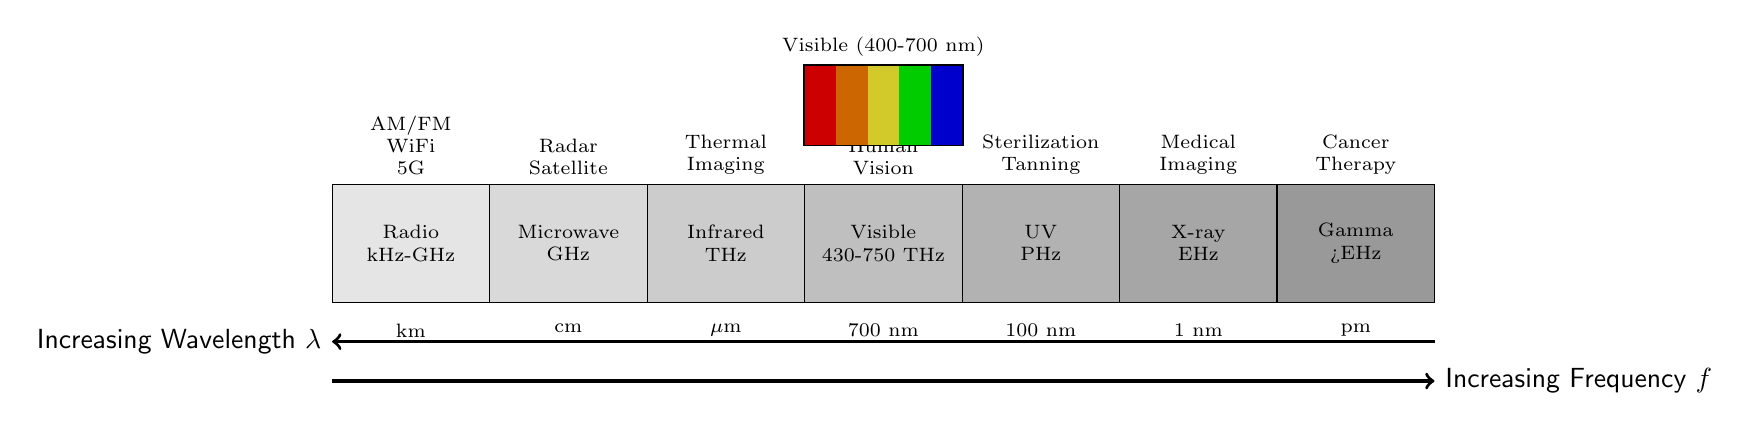
\begin{tikzpicture}[scale=1.0]
% Frequency axis (logarithmic scale representation)
\draw[->,very thick] (0,0) -- (14,0) node[right] {\sffamily Increasing Frequency $f$};
\draw[->,very thick] (14,0.5) -- (0,0.5) node[left] {\sffamily Increasing Wavelength $\lambda$};

% Spectrum bands (approximate logarithmic spacing)
\draw[fill=black!10] (0,1) rectangle (2,2.5) node[pos=0.5,align=center,font=\scriptsize] {Radio\\kHz-GHz};
\draw[fill=black!15] (2,1) rectangle (4,2.5) node[pos=0.5,align=center,font=\scriptsize] {Microwave\\GHz};
\draw[fill=black!20] (4,1) rectangle (6,2.5) node[pos=0.5,align=center,font=\scriptsize] {Infrared\\THz};
\draw[fill=black!25] (6,1) rectangle (8,2.5) node[pos=0.5,align=center,font=\scriptsize] {Visible\\430-750~THz};
\draw[fill=black!30] (8,1) rectangle (10,2.5) node[pos=0.5,align=center,font=\scriptsize] {UV\\PHz};
\draw[fill=black!35] (10,1) rectangle (12,2.5) node[pos=0.5,align=center,font=\scriptsize] {X-ray\\EHz};
\draw[fill=black!40] (12,1) rectangle (14,2.5) node[pos=0.5,align=center,font=\scriptsize] {Gamma\\>EHz};

% Wavelength labels - positioned below rectangles to avoid overlap
\node[below,font=\scriptsize] at (1,0.85) {km};
\node[below,font=\scriptsize] at (3,0.85) {cm};
\node[below,font=\scriptsize] at (5,0.85) {$\mu$m};
\node[below,font=\scriptsize] at (7,0.85) {700~nm};
\node[below,font=\scriptsize] at (9,0.85) {100~nm};
\node[below,font=\scriptsize] at (11,0.85) {1~nm};
\node[below,font=\scriptsize] at (13,0.85) {pm};

% Applications
\node[above,font=\scriptsize,align=center] at (1,2.5) {AM/FM\\WiFi\\5G};
\node[above,font=\scriptsize,align=center] at (3,2.5) {Radar\\Satellite};
\node[above,font=\scriptsize,align=center] at (5,2.5) {Thermal\\Imaging};
\node[above,font=\scriptsize,align=center] at (7,2.5) {Human\\Vision};
\node[above,font=\scriptsize,align=center] at (9,2.5) {Sterilization\\Tanning};
\node[above,font=\scriptsize,align=center] at (11,2.5) {Medical\\Imaging};
\node[above,font=\scriptsize,align=center] at (13,2.5) {Cancer\\Therapy};

% Visible light detail box
\draw[very thick] (6,3) rectangle (8,4);
\fill[red!80!black] (6,3) rectangle (6.4,4);
\fill[orange!80!black] (6.4,3) rectangle (6.8,4);
\fill[yellow!80!black] (6.8,3) rectangle (7.2,4);
\fill[green!80!black] (7.2,3) rectangle (7.6,4);
\fill[blue!80!black] (7.6,3) rectangle (8,4);
\node[above,font=\scriptsize] at (7,4) {Visible (400-700~nm)};

\end{tikzpicture}
\end{center}

\subsection{Frequency Bands and Applications}

{\def\LTcaptype{} % do not increment counter
\begin{longtable}[]{@{}llll@{}}
\toprule\noalign{}
Band & Frequency & Wavelength & Applications \\
\midrule\noalign{}
\endhead
\bottomrule\noalign{}
\endlastfoot
\textbf{ELF} & 3-30 Hz & 10,000-100,000 km & Submarine communication \\
\textbf{VLF} & 3-30 kHz & 10-100 km & Navigation \\
\textbf{LF} & 30-300 kHz & 1-10 km & AM radio \\
\textbf{MF} & 300 kHz-3 MHz & 100-1000 m & AM broadcast \\
\textbf{HF} & 3-30 MHz & 10-100 m & Shortwave \\
\textbf{VHF} & 30-300 MHz & 1-10 m & FM radio, TV \\
\textbf{UHF} & 300 MHz-3 GHz & 10 cm-1 m & Cell phones, WiFi \\
\textbf{SHF} & 3-30 GHz & 1-10 cm & Radar, satellite \\
\textbf{EHF} & 30-300 GHz & 1-10 mm & mmWave, 5G \\
\textbf{THz} & 0.3-3 THz & 0.1-1 mm & Imaging, spectroscopy \\
\textbf{IR} & 300 THz-430 THz & 700 nm-1 mm & Thermal imaging \\
\textbf{Visible} & 430-750 THz & 400-700 nm & Human vision \\
\textbf{UV} & 750 THz-30 PHz & 10-400 nm & Sterilization \\
\textbf{X-ray} & 30 PHz-30 EHz & 0.01-10 nm & Medical imaging \\
\textbf{Gamma} & \textgreater{} 30 EHz & \textless{} 0.01 nm & Nuclear medicine \\
\end{longtable}
}

\textbf{All obey Maxwell's equations!} (though quantum effects become important at high frequencies)

\section{Maxwell's Equations: Conceptual Flow}

The four Maxwell's equations interconnect to predict electromagnetic waves:

\begin{center}
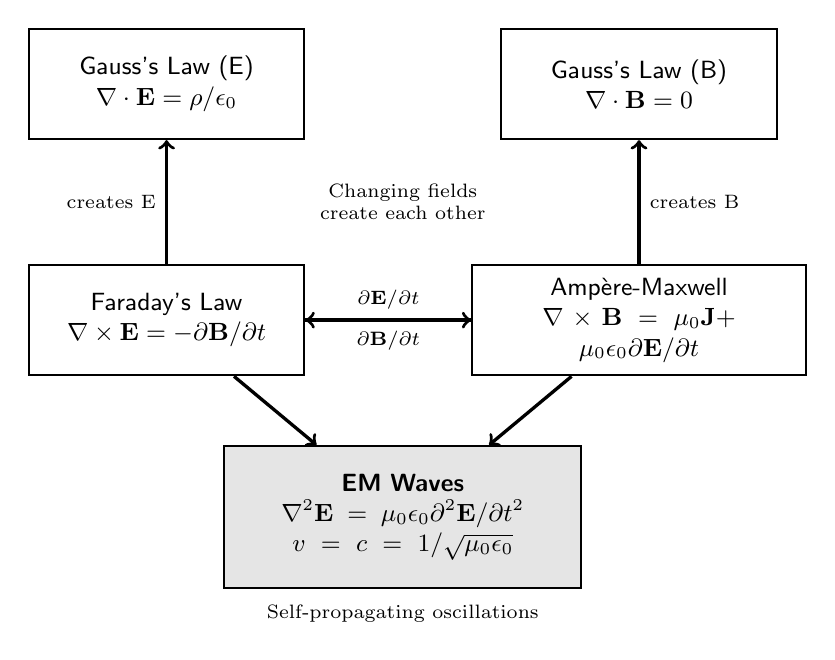
\begin{tikzpicture}[
  box/.style={rectangle, draw, minimum width=3.5cm, minimum height=1.4cm, font=\sffamily\small, align=center, thick},
  node distance=2.5cm
]

% Four equations as boxes
\node[box] (gauss-e) at (0,3) {Gauss's Law (E)\\$\nabla \cdot \mathbf{E} = \rho/\epsilon_0$};
\node[box] (gauss-b) at (6,3) {Gauss's Law (B)\\$\nabla \cdot \mathbf{B} = 0$};
\node[box] (faraday) at (0,0) {Faraday's Law\\$\nabla \times \mathbf{E} = -\partial \mathbf{B}/\partial t$};
\node[box, minimum width=4.2cm, text width=4cm] (ampere) at (6,0) {Ampère-Maxwell\\$\nabla \times \mathbf{B} = \mu_0\mathbf{J} +$\\$\mu_0\epsilon_0 \partial \mathbf{E}/\partial t$};

% Central result - adjusted size for better readability
\node[box, fill=black!10, minimum width=4.5cm, minimum height=1.8cm, text width=4.3cm] (waves) at (3,-2.5) {\textbf{EM Waves}\\$\nabla^2 \mathbf{E} = \mu_0\epsilon_0 \partial^2 \mathbf{E}/\partial t^2$\\$v = c = 1/\sqrt{\mu_0\epsilon_0}$};

% Arrows showing relationships
\draw[->,very thick] (faraday) -- (gauss-e) node[midway,left,font=\scriptsize] {creates E};
\draw[->,very thick] (ampere) -- (gauss-b) node[midway,right,font=\scriptsize] {creates B};
\draw[->,very thick] (faraday) -- (ampere) node[midway,below,font=\scriptsize] {$\partial \mathbf{B}/\partial t$};
\draw[->,very thick] (ampere) -- (faraday) node[midway,above,font=\scriptsize] {$\partial \mathbf{E}/\partial t$};

% To waves
\draw[->,very thick] (faraday) -- (waves);
\draw[->,very thick] (ampere) -- (waves);

% Labels
\node[font=\scriptsize,align=center] at (3,1.5) {Changing fields\\create each other};
\node[font=\scriptsize,align=center,below] at (3,-3.5) {Self-propagating oscillations};

\end{tikzpicture}
\end{center}

\begin{calloutbox}{The Feedback Loop}
Maxwell's equations reveal a remarkable feedback mechanism: changing magnetic fields create electric fields (Faraday), and changing electric fields create magnetic fields (Ampère-Maxwell). This mutual creation allows disturbances to propagate as self-sustaining waves through empty space.
\end{calloutbox}

\section{Applications}

\subsection{Wireless Communications}

\textbf{All wireless technologies rely on Maxwell's equations:}
\begin{itemize}
\item \textbf{Radio/TV Broadcasting:} AM (kHz-MHz), FM (88-108~MHz)
\item \textbf{Mobile Networks:} 4G LTE (700~MHz-2.6~GHz), 5G (sub-6~GHz and mmWave 24-40~GHz)
\item \textbf{WiFi:} 2.4~GHz and 5~GHz bands
\item \textbf{Bluetooth:} 2.4~GHz ISM band
\item \textbf{GPS:} L1 (1575~MHz), L2 (1227~MHz)
\item \textbf{Satellite:} C-band (4-8~GHz), Ku-band (12-18~GHz), Ka-band (26-40~GHz)
\end{itemize}

\subsection{Radar and Sensing}

\begin{itemize}
\item \textbf{Weather Radar:} S-band (2-4~GHz), C-band (4-8~GHz)
\item \textbf{Automotive Radar:} 24~GHz (legacy), 77-81~GHz (modern)
\item \textbf{Airport Security:} mmWave scanners (24-30~GHz)
\item \textbf{Remote Sensing:} Synthetic Aperture Radar (SAR) for Earth observation
\end{itemize}

\subsection{Medical Applications}

\begin{itemize}
\item \textbf{MRI:} Uses RF pulses (10-500~MHz) to manipulate nuclear spins
\item \textbf{Diathermy:} Microwave heating (915~MHz, 2.45~GHz) for physical therapy
\item \textbf{X-ray Imaging:} High-energy EM waves for diagnostic imaging
\item \textbf{Radiation Therapy:} Gamma rays for cancer treatment
\end{itemize}

\subsection{Optical Technologies}

\begin{itemize}
\item \textbf{Fiber Optics:} Near-infrared (1310~nm, 1550~nm) for long-distance communication
\item \textbf{LiDAR:} Pulsed laser (typically 905~nm or 1550~nm) for ranging
\item \textbf{Spectroscopy:} Analyzing material composition via absorption/emission spectra
\end{itemize}

\section{Summary and Key Insights}

\begin{keyconcept}
\textbf{Key Insights from Maxwell's Equations:}
\begin{enumerate}
\item \textbf{Unification:} Electricity, magnetism, and light are different manifestations of the same electromagnetic phenomenon
\item \textbf{Self-propagation:} EM waves don't need a medium (unlike sound)---they can travel through vacuum
\item \textbf{Universal speed limit:} $c$ is the maximum speed in the universe (foundation of special relativity)
\item \textbf{Transverse waves:} $\mathbf{E}$, $\mathbf{B}$, and propagation direction $\hat{\mathbf{k}}$ are mutually perpendicular
\item \textbf{Field duality:} $\mathbf{E}$ and $\mathbf{B}$ are inseparable---changing one creates the other
\item \textbf{Scale invariance:} Same equations govern radio waves through gamma rays (though quantum effects matter at high frequencies)
\end{enumerate}
\end{keyconcept}

\section{Further Reading}

\begin{itemize}
\item \textbf{Electromagnetic-Spectrum}---Detailed frequency breakdown and band allocations
\item \textbf{Antenna-Theory-Basics}---How to efficiently radiate and receive EM waves
\item \textbf{Wave-Polarization}---Electric field orientation and applications
\item \textbf{Free-Space-Path-Loss-(FSPL)}---How wave intensity decreases with distance
\item \textbf{Terahertz-(THz)-Technology}---Emerging applications in the THz gap
\end{itemize}

\section{References}

\begin{enumerate}
\def\labelenumi{\arabic{enumi}.}
\tightlist
\item
  \textbf{Maxwell, J.C.} (1865) ``A Dynamical Theory of the
  Electromagnetic Field'' \emph{Phil. Trans. R. Soc.} 155, 459-512
\item
  \textbf{Jackson, J.D.} (1999) \emph{Classical Electrodynamics} 3rd
  ed.~(Wiley)
\item
  \textbf{Griffiths, D.J.} (2017) \emph{Introduction to Electrodynamics}
  4th ed.~(Cambridge UP)
\item
  \textbf{Feynman, R.P., Leighton, R.B., Sands, M.} (1964) \emph{The
  Feynman Lectures on Physics} Vol. 2 (Addison-Wesley)
\end{enumerate}
